\subsection{SCRUM}
\label{scrum_sec}

O \emph{Scrum}, segundo \citeonline{Rubin2012}, é um método ágil para desenvolvimento de produtos e serviços inovadores. 
A Figura \ref{scrum_geral} mostra uma visão geral do \emph{Scrum}.
\begin{figure}[ht]
	\centering
	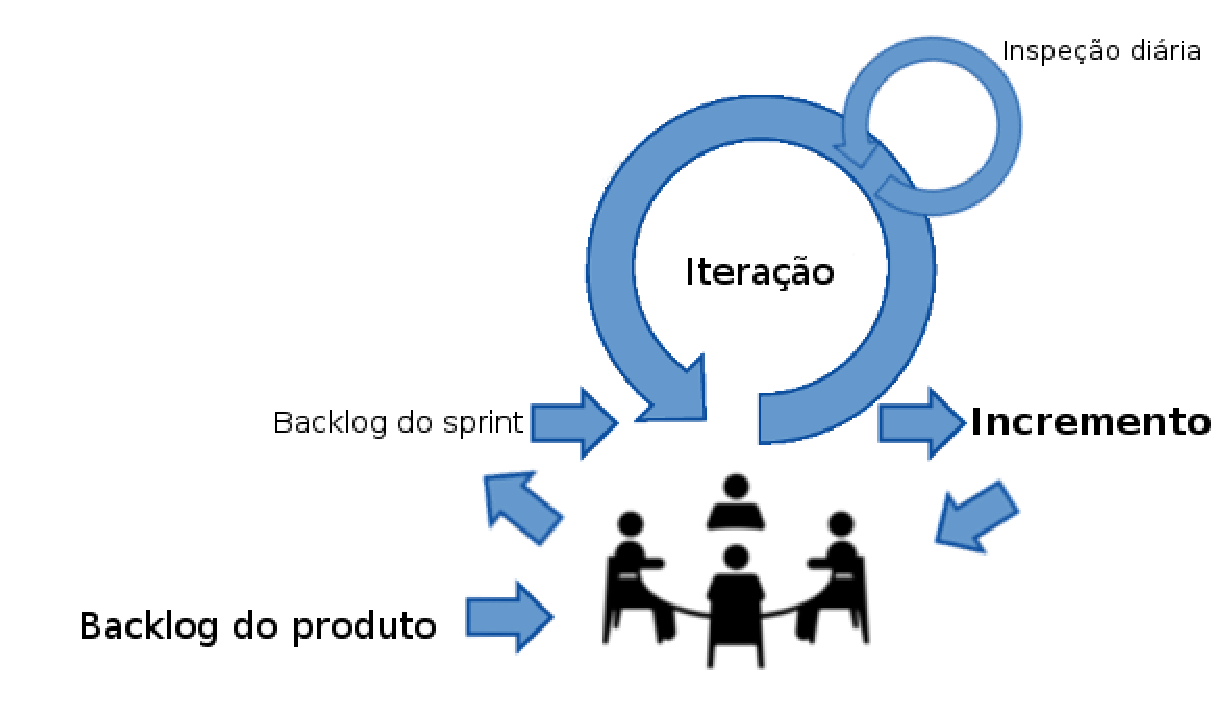
\includegraphics[width=15cm]{figuras/scrum_geral.eps}
	\caption{Visão Geral do \emph{Scrum}. Adaptado de \cite{Schwaber2004}.}
	\label{scrum_geral}
\end{figure}

Basicamente, o fluxo do scrum consiste na criação de um \emph{backlog} de produto. 
Este \emph{backlog} é uma lista de requisitos a serem implementados no processo de desenvolvimento, e é mantido e priorizado pelo \emph{product owner}. 
A lista em si pode receber contribuições dos mais diversos envolvidos no processo, mas a última palavra na priorização é sempre do \emph{product owner}.
A orientação mais aceita para a priorização dos requisitos, é levar em conta aqueles que mais gerarão valor para o usuário final, no momento em questão \cite{Schwaber2001}.

A próxima etapa no fluxo é a reunião de \emph{sprint}. 
Esta reunião consiste na demonstração das funcionalidades implementadas na última iteração e na seleção das funcionalidades que serão construídas na próxima iteração.
As funcionalidades são escolhidas pelos desenvolvedores, que se comprometem a entregá-las ao final da iteração \cite{Schwaber2004}.

Após a reunião do \emph{sprint}, inicia-se a iteração. A iteração é também chamada de \emph{sprint} e consiste num prazo de alguns dias ou alguns meses. 
Isto depende do projeto em questão. Geralmente \emph{sprints} menores são mais aconselhados, uma semana por exemplo \cite{Schwaber2004}.

Durante a iteração ou \emph{sprint}, ao final do dia preferencialmente, realiza-se uma reunião de inspeção diária. 
Esta reunião é também chamada de \emph{daily scrum}. 
Nesta reunião, os envolvidos diretamente no desenvolvimento do produto ou serviço, expõe o andamento de suas atividades pessoais e os impedimentos para a conclusão destas. 
A reunião é feita com todos de pé, e cada um dispõe apenas de alguns minutos de exposição, por exemplo, 3 minutos. 
A intromissão de pessoas externas deve ser evitada. 
A ideia é manter a objetividade e o foco nas tarefas do \emph{sprint}.
Ao final da reunião o \emph{scrum master} deve procurar intender todos os impedimentos expostos. A partir deste conhecimento ele deve tomar medidas necessárias para removê-los, assim garantindo o bom funcionamento da equipe de desenvolvimento.
Ao final do \emph{sprint} um incremento, ou seja, um pedaço de software com funcionalidades implementadas é construído e preferencialmente implantado. O próximo passo é uma nova reunião de \emph{sprint}.

Os papéis definidos pelo \emph{scrum} são \cite{Schwaber2004}:
\begin{itemize}	
	\item \emph{Product Owner};
	\item \emph{Scrum Master};
	\item Desenvolvedor.
\end{itemize}

Nas organizações existirão outros papeis, como gerentes, diretores, patrocinadores, usuários finais, entre outros. 
O importante a se observar, é que apenas os três papeis, \emph{product owner}, \emph{scrum master} e desenvolvedor, é que fazem parte da equipe \emph{scrum}. 
Os demais papeis participam do projeto, mas é necessário, o entendimento por parte da organização, que demandas de implementação devem ser colocadas no backlog do produto. 
Só o \emph{product owner} pode priorizar os novos requisitos. 
Sem este entendimento e comprometimento, fica inviável respeitar prazos e escopo, tornando o processo caótico \cite{Schwaber2004}.

Devido ao \emph{Scrum} servir de espinha dorsal a um processo de desenvolvimento ágil, também sendo amplamente utilizado pelo mercado de desenvolvimento de software, ele foi selecionado como método de gestão deste trabalho. 
Todo o processo do \emph{Scrum} pode ser minunciosamente estudado em \citeonline{Schwaber2001}.


